\documentclass{article}

\usepackage{geometry}
\geometry{margin=2cm}
\usepackage{graphicx}
\usepackage{hyperref}
\usepackage{amsfonts}
\usepackage{caption}
\usepackage{subcaption}

\hypersetup{colorlinks=true, linkcolor=blue, urlcolor=blue}
\urlstyle{same}
\begin{document}
	
	\author{Aayush Arya}
	\date{(Submitted: \today)}
	\title{}
	
	\maketitle
	
	\hrule
	\begin{center}
		PHY350 Lab Report\\
		Practical: 9 \quad Registration No.: 11912610 \quad Section: G2903
	\end{center}
	\hrule
	
	\section*{Aim}
	To measure high resistance using leakage method
	
	\section*{Results \& Conclusions}
	
	We obtained an estimate of $R$ by finding an average slope to the data points (see Figure \ref{fig:out}). The slope of $\log_{10}\left(\frac{\theta_0}{\theta_t}\right)$ vs time plot is found using least squares fitting.
	
	The resistance we obtained was $R \sim 8.14 \times 10^6 \Omega$, which corresponds to a percentage error of $-1.85\%$ from the true value. 
	
	\begin{figure}[h!]
		\centering
		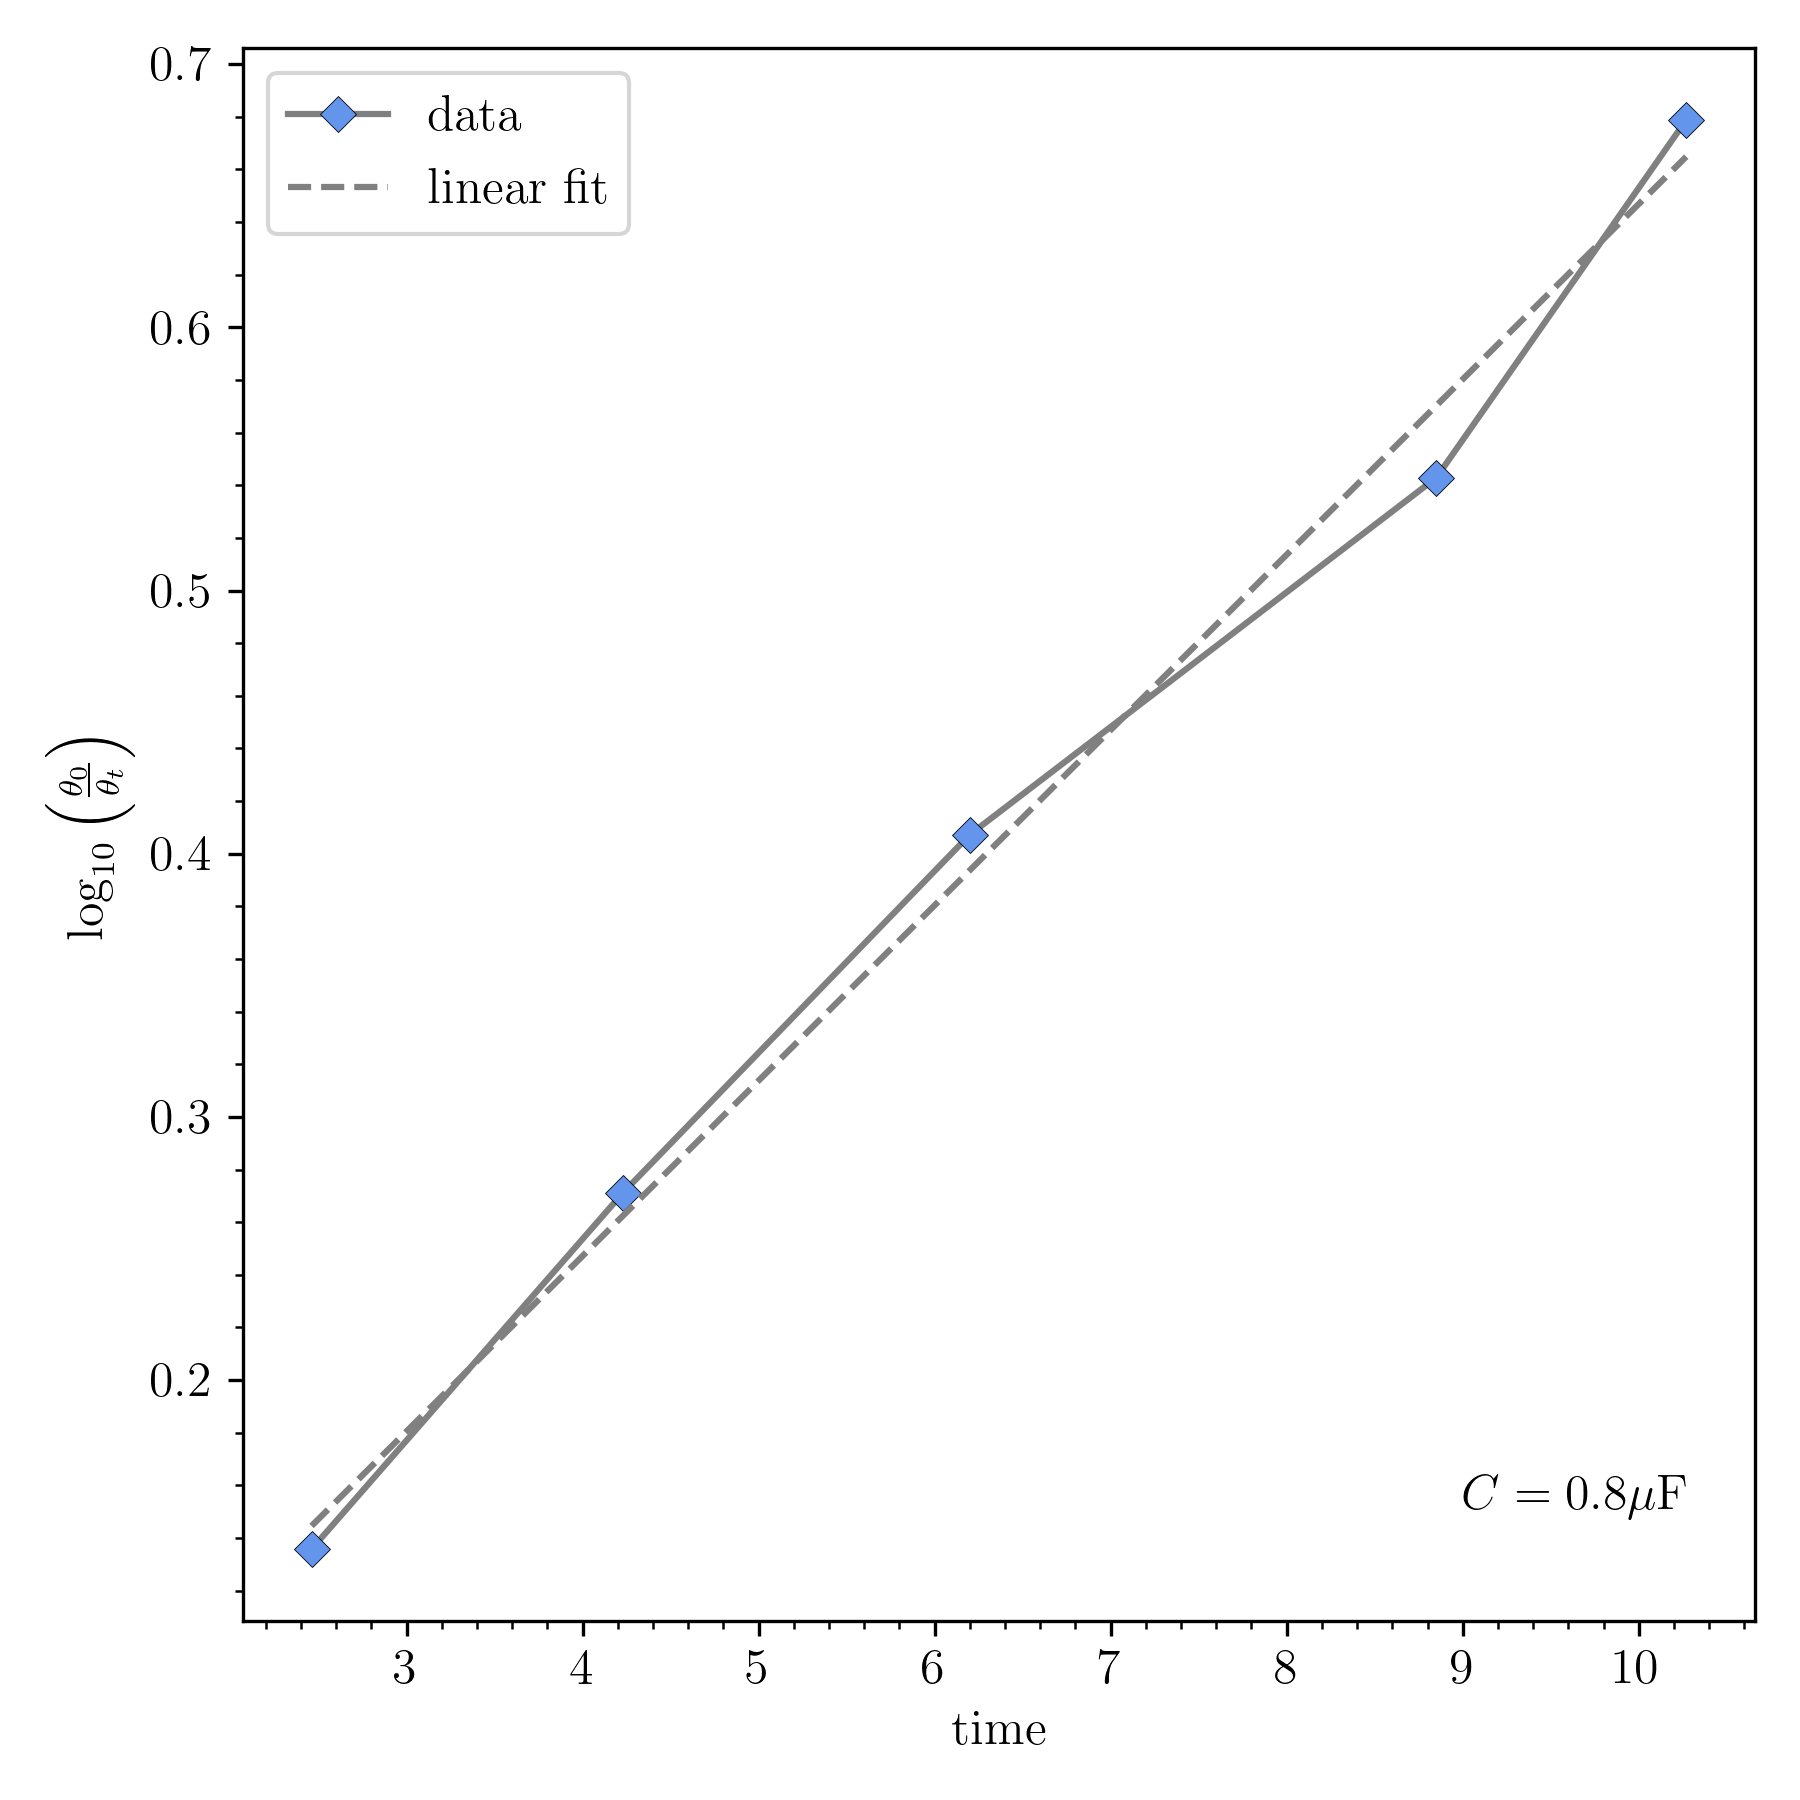
\includegraphics[width=0.7\textwidth]{prac9_plot}
		\caption{The straight line fit done using a least squares regression is shown with a dashed line.}
		\label{fig:out}
	\end{figure}
	
	Due to the relation \[\log_{10}\left(\frac{\theta_0}{\theta_t}\right) = \frac{t}{2.303 RC}\] the slope is related to the resistance as \[R = \frac{1}{2.303mC}\]
	
	The measurements for the output characteristics have been summarized in Table \ref{tab:out}.
	
	\begin{table}[!h]
		\centering
		\begin{tabular}{|c|c|c|c|c|}
			\hline
			$\theta_0$ & Discharging time & $\theta_t$ & $\theta_0/\theta_t$ & $\log_{10}\theta_0/\theta_t$ \\
			\hline
			20         & 2.46             & 14.63      & 1.37   & 0.14          \\
			20         & 4.23             & 10.71      & 1.87  & 0.27           \\
			20         & 6.2              & 7.83       & 2.55   & 0.40           \\
			20         & 8.85             & 5.73       & 3.49   & 0.54           \\
			20         & 10.27            & 4.19       & 4.77    & 0.68 \\
			\hline         
		\end{tabular}
	\caption{Measurements}
	\label{tab:out}
	\end{table}
	
\end{document}